\documentclass[english,serif,mathserif,xcolor=pdftex,dvipsnames,table]{beamer}
\usepackage{gc3}

\title[Sequences, Iteration]{%
  Sequences and iteration in Python
}
\author[GC3]{%
  GC3: Grid Computing Competence Center, \\
  University of Zurich
}
\date{Mar.~12--13, 2013}

\begin{document}

% title frame
\maketitle


\begin{frame}
  \frametitle{Sequences}
  
  Python provides a few built-in \emph{sequence} classes:
  \begin{description}
  \item[list] \emph{mutable}, possibly heterogeneous
  \item[tuple] \emph{immutable}, possibly heterogeneous
  \item[str] \emph{immutable}, only holds characters
  \end{description}
  Additional sequence types are provided by external modules. For
  instance,  the
  \href{http://numpy.scipy.org}{NumPy} package, which is commonly used in
  scientific Python codes, defines:
  \begin{description}
  \item[array] \emph{mutable}, homogeneous
  \end{description}

\end{frame}




\begin{frame}[fragile]
  \frametitle{Lists - \textit{(mutable, heterogeneous)}}
  Lists are by far the most common and used sequence type in Python.

  \+
  Lists are created and initialized by enclosing values into
  `\texttt{[}' and `\texttt{]}':
\begin{lstlisting}
>>> L = [ 'G', 'C' ]
\end{lstlisting}

  \+
  You can append and remove items from a list:
\begin{lstlisting}
>>> L.append('3')
>>> print (L)
['G', 'C', '3']
\end{lstlisting}

  \+
  You can append \textbf{any} object to it:
\begin{lstlisting}
>>> L.append(L)
>>> print(L)
['G', 'C', '3', [...]]
\end{lstlisting}

  % % \+
  % \begin{references}
  %   \url{http://docs.python.org/tutorial/datastructures.html#more-on-lists}
  % \end{references}
\end{frame}


\begin{frame}[fragile,fragile]
  \frametitle{Sequences, II}
  You can access individual items in a sequence using the postfix
  \texttt{[]} operator.

  \+
  Sequence indices start at 0.
\begin{lstlisting}
>>> L = ['G', 'C', '3']
>>> print L[0], L[1], L[2]
'G' 'C' '3'
>>> S = 'GC3'
>>> print S[0], S[1], S[2]
'G' 'C' '3'
\end{lstlisting}

  \+
  The \texttt{len()} function returns the number of elements in a
  sequence.
\begin{lstlisting}
>>> len(L)
3
\end{lstlisting}
\end{frame}


\begin{frame}[fragile]
  \frametitle{Slices}
  The notation \texttt{[$n$:$m$]} is used for accessing a \emph{slice}
  of sequence (the items at positions $n$, $n+1$, \ldots, $m-1$).
\begin{lstlisting}
>>> # list numbers from 0 to 9
>>> R = range(0,10)
>>> R[1:4]
[1, 2, 3]
\end{lstlisting}

  \+
  If $n$ is omitted it defaults to 0, if $m$ is omitted it defaults to
  the length of the sequence.
\end{frame}


\begin{frame}[fragile]
  \frametitle{List mutation}
  You can replace items in a \emph{mutable} sequence by assigning them
  a new value:
\begin{lstlisting}
>>> L[2] = 'Z'
>>> print L
['G', 'C', 'Z']
\end{lstlisting}

  You can also replace an entire slice of a mutable sequence:
\begin{lstlisting}
>>> L[1:3] = [1, 2, 3]
>>> print L
['G', 1, 2, 3]
\end{lstlisting}
  The new slice does not need to have the same length:
\begin{lstlisting}
>>> L[1:] = 'Zurich'
>>> print L
['G', 'Z', 'u', 'r', 'i', 'c', 'h']
\end{lstlisting}
\end{frame}


\begin{frame}[fragile]
  \frametitle{Dictionaries}
  The \texttt{dict} type implements a key/value mapping:
\begin{lstlisting}
>>> D = { }
>>> D['a'] = 1
>>> D[2] = 'b'
>>> D
{'a': 1, 2: 'b'}
\end{lstlisting}

  \+
  Dictionaries can be created and initialized using two
  different but equivalent syntaxes:
\begin{lstlisting}
>>> D1 = { 'a':1, 'b':2 }
>>> D2 = dict(a=1, b=2)
>>> D1 == D2
True
\end{lstlisting}
\end{frame}


\begin{frame}[fragile]
  \frametitle{Sets}
  The \texttt{set} type implements an unordered container that holds
  exactly one object per equivalence class:
\begin{lstlisting}
>>> S = set()
>>> S.add(1)
>>> S.add(2)
>>> S.add(1)
>>> S
set([1, 2])
\end{lstlisting}

  \+
  You can create a set and add elements to it in one go:
\begin{lstlisting}
>>> S2 = set([1, 2])
>>> S2 == S
True
\end{lstlisting}
\end{frame}


\begin{frame}[fragile]
  \frametitle{Mutable vs Immutable}
  Some objects (e.g., \texttt{tuple}, \texttt{int}, \texttt{str})
  are \emph{immutable} and cannot be modified.
\begin{lstlisting}[basicstyle=\footnotesize\ttfamily]
>>> T = ('U', 'Z', 'H')
>>> T[2] = 'h'
Traceback (most recent call last):
  File "<stdin>", line 1, in <module>
TypeError: 'tuple' object does not support item assignment
\end{lstlisting}

\+
\begin{lstlisting}
>>> S = 'GC3'
>>> S[2] = '2'
Traceback (most recent call last):
  File "<stdin>", line 1, in <module>
TypeError: 'str' object does not support item assignment
\end{lstlisting}

  
  \+
  \texttt{list}, \texttt{dict}, \texttt{set} and user-defined objects
  are \emph{mutable} and can be modified in-place.
\end{frame}



\begin{frame}[fragile]
  \frametitle{The `{\ttfamily\bfseries in}' operator}
  
  Use the \lstinline|in| operator to test for presence of an item in a
  collection.

  \begin{describe}{\lstinline|x in S|}
    Evaluates to \texttt{True} if \lstinline|x| is equal to a \emph{value}
    contained in the \lstinline|S| sequence (list, tuple, set).
  \end{describe}
  
  \begin{describe}{\lstinline|x in D|}
    Evaluates to \texttt{True} if \lstinline|x| is equal to a \emph{key}
    in the \lstinline|D| dictionary.
  \end{describe}
  
  \begin{describe}{\lstinline|x in T|}
    Evaluates to \texttt{True} if \lstinline|x| is a substring of
    string \lstinline|T|.
  \end{describe}
  
\end{frame}


\begin{frame}[fragile,fragile]
  \frametitle{The \texttt{in} operator and the \texttt{if} conditional
  }
  
  To test if a specific element is present in a sequence, use the
  \texttt{in} operator:

\begin{lstlisting}
>>> L = [1, 2, 3, 4]
>>> if 1 in L:
...   print "Found!"
...
Found!
\end{lstlisting}

\+
And it works with \textbf{any} sequence:
\begin{lstlisting}
>>> if 'a' in ('a', 'b', 'c'):
...    print "Found!"
Found!
>>> if 'key' in {'key': 'value', 'key2': 'value'}:
...    print "Key found!"
Key found!
\end{lstlisting}
\end{frame}

% \begin{frame}[fragile]
%   \frametitle{Useful data structures operations}

%   Read {\url{http://docs.python.org/tutorial/datastructures.html}}.

%   \+
%   Really, you will need it.

%   \+
%   And remember that \texttt{dir()} and \texttt{help()} are your friends!
% \end{frame}


\begin{frame}[fragile]
  \frametitle{All variables are references}

  In Python, \textbf{all objects are ever passed by reference}.

  \+
  In particular, \textbf{variables always store a reference to an
    object}, never a copy!

  \+
  Hence, you have to be careful when modifying objects:
\begin{lstlisting}
>>> a = [1,2,3]
>>> b = a
>>> b.remove(2)
>>> print a
[1, 3]
\end{lstlisting}

   \+
   \href{http://tinyurl.com/cq3tcab}{Run this example} in the
   \href{http://pythontutor.com/}{Online Python Tutor} to better
   understand what's going on.

   \+
   {\small \em
     This applies particularly for variables that capture the arguments
     to a function call!}

\end{frame}


\begin{frame}[fragile]
  \frametitle{All variables are references (demo)}
  \href{http://www.pythontutor.com/}{www.pythontutor.com}

  \only<1>{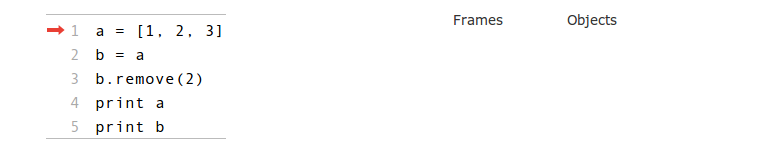
\includegraphics[width=1.2\textheight]{t1_screenshot_1.png}}
  \only<2>{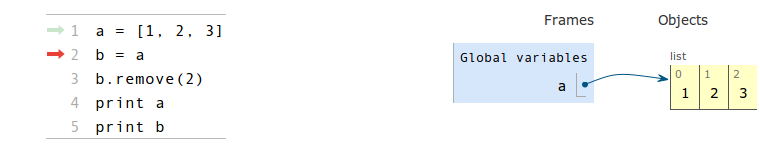
\includegraphics[width=1.2\textheight]{t1_screenshot_2.png}}
  \only<3>{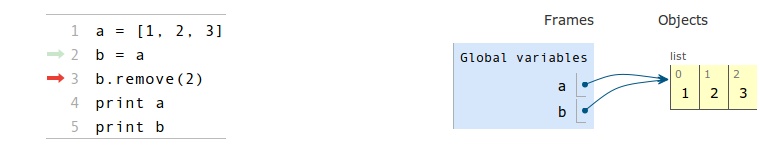
\includegraphics[width=1.2\textheight]{t1_screenshot_3.png}}
  \only<4>{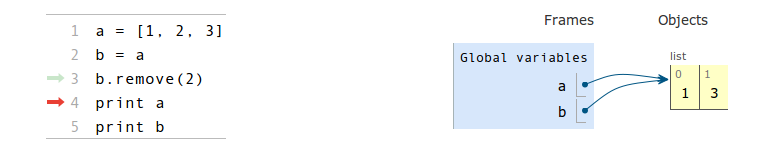
\includegraphics[width=1.2\textheight]{t1_screenshot_4.png}}
\end{frame}

%%%%%%%%%%%%%%%%%%%%%%%%%%%%%%%%%%%%%%%%%%%%%%%%%%%%%%%%%%%%%%%%%%
% I'm removing this slide because this does not always work. For %
% lists, for instances, it doesn't work as expected:             %
%                                                                %
% >>> l = range(3)                                               %
% >>> a = range(3)                                               %
% >>> b = a                                                      %
% >>> a                                                          %
% [0, 1, 2]                                                      %
% >>> b+= [4]                                                    %
% >>> a                                                          %
% [0, 1, 2, 4]                                                   %
% >>> b                                                          %
% [0, 1, 2, 4]                                                   %
%%%%%%%%%%%%%%%%%%%%%%%%%%%%%%%%%%%%%%%%%%%%%%%%%%%%%%%%%%%%%%%%%%
%
% \begin{frame}[fragile]
%   \frametitle{All variables are references, II}
%   \emph{However:}
% \begin{lstlisting}
% >>> a = 1
% >>> b = a
% >>> b += 1
% >>> a
% 1
% >>> b
% 2
% \end{lstlisting}
%   \begin{question}
%     How can you explain this? 

%     \pause{The \texttt{b += 1} operator could be replaced by
%       \texttt{b = b + 1}, and the \texttt{b+1} expression yields a
%       \emph{new} value.}
%   \end{question}
% \end{frame}


\begin{frame}[fragile]
  \frametitle{\texttt{for}-loops}
    With the  \texttt{for} statement, you can loop over the values in
    a list:
\begin{lstlisting}
for i in range(0, 4):
  # loop block
  print (i*i)
\end{lstlisting}

  \+
  To break out of a \texttt{for} loop, use the \texttt{break}
  statement.

  \+
  To jump to the next iteration of a \texttt{for} loop, use the
  \texttt{continue} statement.
\end{frame}


\begin{frame}[fragile]
  The \texttt{for} statement can be used to loop over elements in \emph{any sequence}.

  \+
  \begin{columns}[c]
    \begin{column}{0.5\textwidth}
\begin{lstlisting}
>>> for val in @\HL{1,2,3}@:
...   print val
1
2
3
\end{lstlisting}
    \end{column}
    \begin{column}{0.4\textwidth}
      \raggedleft
      Loop over tuples
    \end{column}
  \end{columns}
\end{frame}

\begin{frame}[fragile]
  The \texttt{for} statement can be used to loop over elements in \emph{any sequence}.

  \+
  \begin{columns}[c]
    \begin{column}{0.5\textwidth}
\begin{lstlisting}
>>> for val in @\HL{'GC3'}@:
...   print val
'G'
'C'
'3'
\end{lstlisting}
    \end{column}
    \begin{column}{0.4\textwidth}
      \raggedleft
      Loop over strings
    \end{column}
  \end{columns}
\end{frame}

\begin{frame}[fragile]
  The \texttt{for} statement can be used to loop over elements in \emph{any sequence}.

  \+
  \begin{columns}[c]
    \begin{column}{0.5\textwidth}
\begin{lstlisting}
>>> D = dict(a=1, b=2)
>>> for val in @\HL{D.keys()}@:
...   print val
'a'
'b'
\end{lstlisting}
    \end{column}
    \begin{column}{0.4\textwidth}
      \raggedleft
      Loop over dictionary~\emph{keys}.

      \emph{The \texttt{.keys()} part can be omitted, as it's the
        default!}
    \end{column}
  \end{columns}
\end{frame}

\begin{frame}[fragile]
  If you want to loop over dictionary \emph{values}, you have to
  explicitly request it.

  \+
  \begin{columns}[c]
    \begin{column}{0.5\textwidth}
\begin{lstlisting}
>>> D = dict(a=1, b=2)
>>> for val in @\HL{D.values()}@:
...   print val
1
2
\end{lstlisting}
    \end{column}
    \begin{column}{0.4\textwidth}
      \raggedleft
      Loop over dictionary~\emph{values}

      \emph{The \texttt{.values()} cannot be omitted!}
    \end{column}
  \end{columns}
\end{frame}


\begin{frame}[fragile]
  Multiple assignment can be used in \texttt{for} statements as well.
\begin{lstlisting}
>>> L = [(1,'a'), (2,'b'), (3, 'c')]
>>> for num, char in L:
...     print ("num is " + str(num)
...            + ' and char is ' + char)
\end{lstlisting}

  \+
  This is particularly useful with functions that return a tuple.
  For instance the \texttt{enumerate()} function (look it up with
  \texttt{help()}!).
\end{frame}


\begin{frame}
  \begin{exercise}
    Write a function \texttt{invert(D)} that takes a dictionary
    \texttt{D} and returns a dictionary \texttt{Dinv} with keys and
    values swapped. (We assume that \texttt{D} is 1-1.)
  \end{exercise}

  \+
  \begin{exercise}
    Implement a \texttt{zip2} function, that takes a list of 2-tuples
    and returns \emph{two} lists: a list of all the first items in the
    pairs, and a list of all the second items in the pairs.
  \end{exercise}
\end{frame}


\begin{frame}[fragile]
  \frametitle{Default values}
  
  Function arguments can have default values.
\begin{lstlisting}
>>> def hello(name='world'):
...   print ("Hello, " + name)
...
>>> hello()
'Hello, world'
\end{lstlisting}
\end{frame}


\begin{frame}[fragile]
  \frametitle{Variadic functions, I}
  Functions like \texttt{max} and \texttt{min} take a variable number of arguments.

  \+
  That is possible with user-defined functions too.

  \+
  If the last argument is prefixed with a \texttt{*} character,
  Python will make that argument into a \emph{tuple} of arguments
  passed to the function. (Except for the ones that have already been
  assigned names.)
\end{frame}


\begin{frame}[fragile,fragile]
  \frametitle{Variadic functions, II}
\begin{lstlisting}
>>> def varfn1(*args):
...   print args
>>> varfn1(1,2,3)
(1, 2, 3)
\end{lstlisting}

\begin{lstlisting}
>>> def varfn2(a, b, *rest):
...   print rest
>>> varfn1(1,2,3)
(3,)
\end{lstlisting}
\end{frame}


\begin{frame}[fragile]
  \frametitle{Variadic functions, III}
  You can call a function with an argument list that is only
  determined at run time.

  \+
  The unary \texttt{*} operator takes any sequence and makes it
  into a function argument list:
\begin{lstlisting}
>>> L = [1, 2, 3]
>>> max(*L)
3
\end{lstlisting}
\end{frame}


\begin{frame}[fragile]
  \frametitle{Named arguments}
Python allows calling a function with named arguments:
\begin{lstlisting}
hello(name="Alice")
\end{lstlisting}
When passing arguments by name, they can be passed in any order:
\begin{lstlisting}
>>> from fractions import Fraction
>>> Fraction(numerator=1, denominator=2)
Fraction(1, 2)
>>> Fraction(denominator=2, numerator=1)
Fraction(1, 2)
\end{lstlisting}
\end{frame}


\begin{frame}[fragile]
  \frametitle{Keyword arguments, I}
  Python lets you catch arbitrary named arguments.

  \+
  Prefix the very last argument name with \texttt{**}, and Python
  will make it into a dictionary: keys are actual argument names and
  dictionary values are actual argument values.

  \+
\begin{lstlisting}
>>> def kwfn1(**kwargs):
...   print kwargs
>>> kwfn1(a=1, b=2)
{'a':1, 'b':2}
\end{lstlisting}
\end{frame}


\begin{frame}[fragile,fragile]
  \frametitle{Keyword arguments, II}
  Keyword argument can be combined with positional arguments:
\begin{lstlisting}
>>> def kwfn1(x, y, **kwargs):
...   print "x=%s y=%s kwargs=%s" % (x, y, kwargs)
>>> kwfn1(0, 42, a=1, b=2)
x=0 y=42 kwargs={'a':1, 'b':2}
\end{lstlisting}

  \+
  \ldots and also with variadic arguments:
\begin{lstlisting}
>>> def kwfn2(x, *rest, **kwargs):
...   print ("x=%s rest=%s kwargs=%s"
...          % (x, rest, kwargs))
>>> kwfn2(0, 1, 2, 3, a=1, b=2)
x=0 rest=(1, 2, 3) kwargs={'a':1, 'b':2}
\end{lstlisting}
\end{frame}


\begin{frame}[fragile,fragile]
  \frametitle{Keyword arguments, III}
  You can pass to a function a set of keyword arguments that is
  determined only at run time.

  The \texttt{**} operator takes any \emph{dictionary} and turns it
  into the bundle of keyword arguments for a function:
\begin{lstlisting}
>>> D = { 'c':4, 'd':2 }
>>> kwfn2(x=1, **D)
x=1 rest=() kwargs={ 'c':4, 'd':2 }
\end{lstlisting}
\end{frame}


\begin{frame}[fragile]
  \begin{exercise}
    Write a \texttt{maxarg} function, that takes arbitrary keyword
    arguments (but assume the values are all numbers), and returns the
    name of the argument with the largest value.

    \+
    Example:
\begin{lstlisting}
>>> maxarg(a=1, b=2)
'b'
\end{lstlisting}
  \end{exercise}
\end{frame}

\end{document}


%%% Local Variables:
%%% mode: latex
%%% TeX-master: t
%%% End:
